\documentclass{beamer}
\usepackage[utf8]{inputenc}

\usetheme{Madrid}
\usecolortheme{default}
\usepackage{amsmath,amssymb,amsfonts,amsthm}
\usepackage{txfonts}
\usepackage{tkz-euclide}
\usepackage{listings}
\usepackage{adjustbox}
\usepackage{array}
\usepackage{tabularx}
\usepackage{gvv}
\usepackage{lmodern}
\usepackage{circuitikz}
\usepackage{tikz}
\usepackage{graphicx}

\setbeamertemplate{page number in head/foot}[totalframenumber]

\usepackage{tcolorbox}
\tcbuselibrary{minted,breakable,xparse,skins}



\definecolor{bg}{gray}{0.95}
\DeclareTCBListing{mintedbox}{O{}m!O{}}{%
	breakable=true,
	listing engine=minted,
	listing only,
	minted language=#2,
	minted style=default,
	minted options={%
		linenos,
		gobble=0,
		breaklines=true,
		breakafter=,,
		fontsize=\small,
		numbersep=8pt,
		#1},
	boxsep=0pt,
	left skip=0pt,
	right skip=0pt,
	left=25pt,
	right=0pt,
	top=3pt,
	bottom=3pt,
	arc=5pt,
	leftrule=0pt,
	rightrule=0pt,
	bottomrule=2pt,
	toprule=2pt,
	colback=bg,
	colframe=orange!70,
	enhanced,
	overlay={%
		\begin{tcbclipinterior}
			\fill[orange!20!white] (frame.south west) rectangle ([xshift=20pt]frame.north west);
	\end{tcbclipinterior}},
	#3,
}
\lstset{
	language=C,
	basicstyle=\ttfamily\small,
	keywordstyle=\color{blue},
	stringstyle=\color{orange},
	commentstyle=\color{green!60!black},
	numbers=left,
	numberstyle=\tiny\color{gray},
	breaklines=true,
	showstringspaces=false,
}
%------------------------------------------------------------
%This block of code defines the information to appear in the
%Title page
\title %optional
{5.8.39}
\date{January 9, 2025}
%\subtitle{A short story}

\author % (optional)
{Nipun Dasari - EE25BTECH11042}



\begin{document}
	
	\frame{\titlepage}
	\begin{frame}{Question}
		The cost of $2$ pencils and $3$	 erasers is $9rs$ and the cost of $4$ pencils and $6$ erasers is
	$18rs$. Find the cost of each pencil and each eraser.
		
	\end{frame}
	
	
	\begin{frame}{Theoretical Solution}
			Let $x$ and $y$ denote the cost of each pencil and eraser respectively.\\
		By forming the equations we get
		\begin{align}
			\vec{n_1}^\top\vec{x}=c_1\\
			\vec{n_2}^\top\vec{x}=c_2
		\end{align}
		Stacking these gives:
		\begin{align}
			\begin{myvec}{\vec{n_1}^\top \\ \vec{n_2}^\top}\end{myvec}\vec{x}= \begin{myvec}{c_1 \\ c_2}\end{myvec}
		\end{align}
		\begin{align}
			\vec{n_1} = \begin{myvec}{2 \\ 3}\end{myvec} \text{, } \vec{n_1} = \begin{myvec}{4 \\ 6}\end{myvec} \text{, } c_1=9 \text{, } c_2 =18
		\end{align}
	\end{frame}
	\begin{frame}{Theoretical Solution}
		Thus,
		\begin{align}
			\begin{myvec}{2 & 3 \\ 4 & 6}\end{myvec}\begin{myvec}{x\\y}\end{myvec} = \begin{myvec}{9\\18}\end{myvec}
		\end{align}
		The augmented matrix is
		\begin{align}
			\augvec{2}{1}{2 & 3 & 9 \\ 4 & 6 & 18}
		\end{align}
		By row transformations:
		\begin{align}
			\augvec{2}{1}{2 & 3 & 9 \\ 4 & 6 & 18}
			&\xleftrightarrow{\,R_2 \gets R_2-2R_1}
			\augvec{2}{1}{2 & 3 & 9 \\ 0 & 0 & 0}
		\end{align}
		This implies that there exist infinitely many solutions as one row is a linear factor of the other. Both equations lead to the same line.
	\end{frame}
	
	
	\begin{frame}[fragile]
		\frametitle{C Code}
		
		\begin{lstlisting}
		double calculate_y(double x, double a, double b, double c) {
			if (b == 0) {
				// Avoid division by zero for vertical lines
				return 0.0; 
			}
			return (c - a * x) / b;
		}
		\end{lstlisting}
	\end{frame}
	\begin{frame}[fragile]
		\frametitle{Python Code using shared output}
		
		\begin{lstlisting}
		import ctypes
		import numpy as np
		import matplotlib.pyplot as plt
		# --- Load the Shared C Library ---
		# Assumes 'line_solver.so' is in the same directory.
		try:
		line_lib = ctypes.CDLL('./5.8.39.so')
		except OSError as e:
		print("Error: Could not load the shared library 'line_solver.so'.")
		print("Please ensure you have compiled 'line_solver.c' correctly.")
		print(e)
		exit()		
		\end{lstlisting}
	\end{frame}
	
	
	\begin{frame}[fragile]
		\frametitle{Python Code using shared output}
		\begin{lstlisting}
		# --- Define the C function's signature for Python ---
		calculate_y_c = line_lib.calculate_y
		calculate_y_c.argtypes = [ctypes.c_double, ctypes.c_double, ctypes.c_double, ctypes.c_double]
		calculate_y_c.restype = ctypes.c_double
		# --- Define coefficients for BOTH equations ---
		# Equation 1: 2x + 3y = 9
		a1, b1, c1 = 2.0, 3.0, 9.0
		# Equation 2: 4x + 6y = 18
		a2, b2, c2 = 4.0, 6.0, 18.0
		# --- Generate data points using the C function ---
		x_values = np.linspace(0, 5, 100)
		y_values_1 = []
		y_values_2 = []	
		\end{lstlisting}
	\end{frame}
	\begin{frame}[fragile]
		\frametitle{Python Code using shared output}
		\begin{lstlisting}		
		# Call the C function for each x value for both lines
		for x in x_values:
		y1 = calculate_y_c(x, a1, b1, c1)
		y_values_1.append(y1)
		
		y2 = calculate_y_c(x, a2, b2, c2)
		y_values_2.append(y2)
		# --- Plot the Results ---
		plt.figure(figsize=(8, 6))
		# Plot the first line
		plt.plot(x_values, y_values_1, 
		label=f'{int(a1)}x + {int(b1)}y = {int(c1)} (via C)', 
		color='blue', 
		linewidth=2)
		\end{lstlisting}
	\end{frame}
	\begin{frame}[fragile]
		\frametitle{Python Code using shared output}
		\begin{lstlisting}		
			# Plot the second line on top with a different style
			plt.plot(x_values, y_values_2, 
			label=f'{int(a2)}x + {int(b2)}y = {int(c2)} (via C)', 
			color='red', 
			linestyle='--', 
			linewidth=4)
			plt.title('Plotting Two Identical Lines Using a C Function')
			plt.xlabel('Cost of Pencil (x)')
			plt.ylabel('Cost of Eraser (y)')
			plt.grid(True)
			plt.legend()
			plt.show()
		\end{lstlisting}
	\end{frame}
	\begin{frame}[fragile]
		\frametitle{Python Code}
		\begin{lstlisting}
# Plot the first line
plt.plot(x, y1, label='2x + 3y = 9', color='blue', linewidth=4)
# Plot the second line on top of the first one with a different style to show they are identical
plt.plot(x, y2, label='4x + 6y = 18', color='red', linestyle='--', linewidth=2)
# Add titles and labels
plt.title("Both Equations Represent the Same Line")
plt.xlabel("Cost of Pencil (x)")
plt.ylabel("Cost of Eraser (y)")
plt.grid(True)
plt.legend()
plt.tight_layout()
# Save the plot to a file
plt.savefig("Figure_2.png")
		\end{lstlisting}
		
	\end{frame}
	
	
	\begin{frame}{Plot by python using shared output from c}
		\begin{figure}[H]
			\centering
			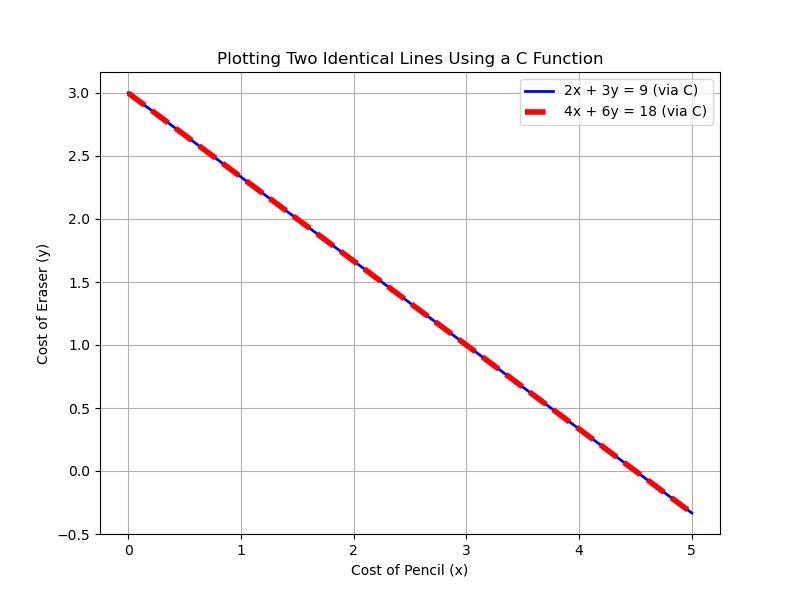
\includegraphics[width = 0.8\columnwidth]{figs/Figure_1.png}
			\caption*{}
			\label{fig1}
		\end{figure}
	\end{frame}
	\begin{frame}{Plot by python}
		\begin{figure}[H]
			\centering
			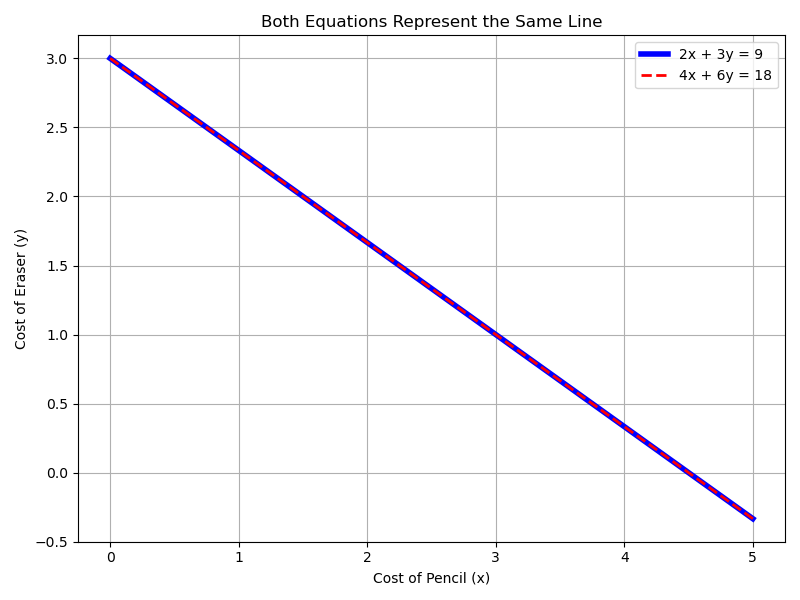
\includegraphics[width = 0.8\columnwidth]{figs/Figure_2.png}
			\caption*{}
			\label{fig2}
		\end{figure}
	\end{frame}
\end{document}